\section{Referencia de la Clase Busqueda\-Trabajador}
\label{classBusquedaTrabajador}\index{BusquedaTrabajador@{BusquedaTrabajador}}
Permite buscar y seleccionar un trabajador.  


{\tt \#include $<$busquedatrabajador.h$>$}

Diagrama de colaboraci\'{o}n para Busqueda\-Trabajador:\begin{figure}[H]
\begin{center}
\leavevmode
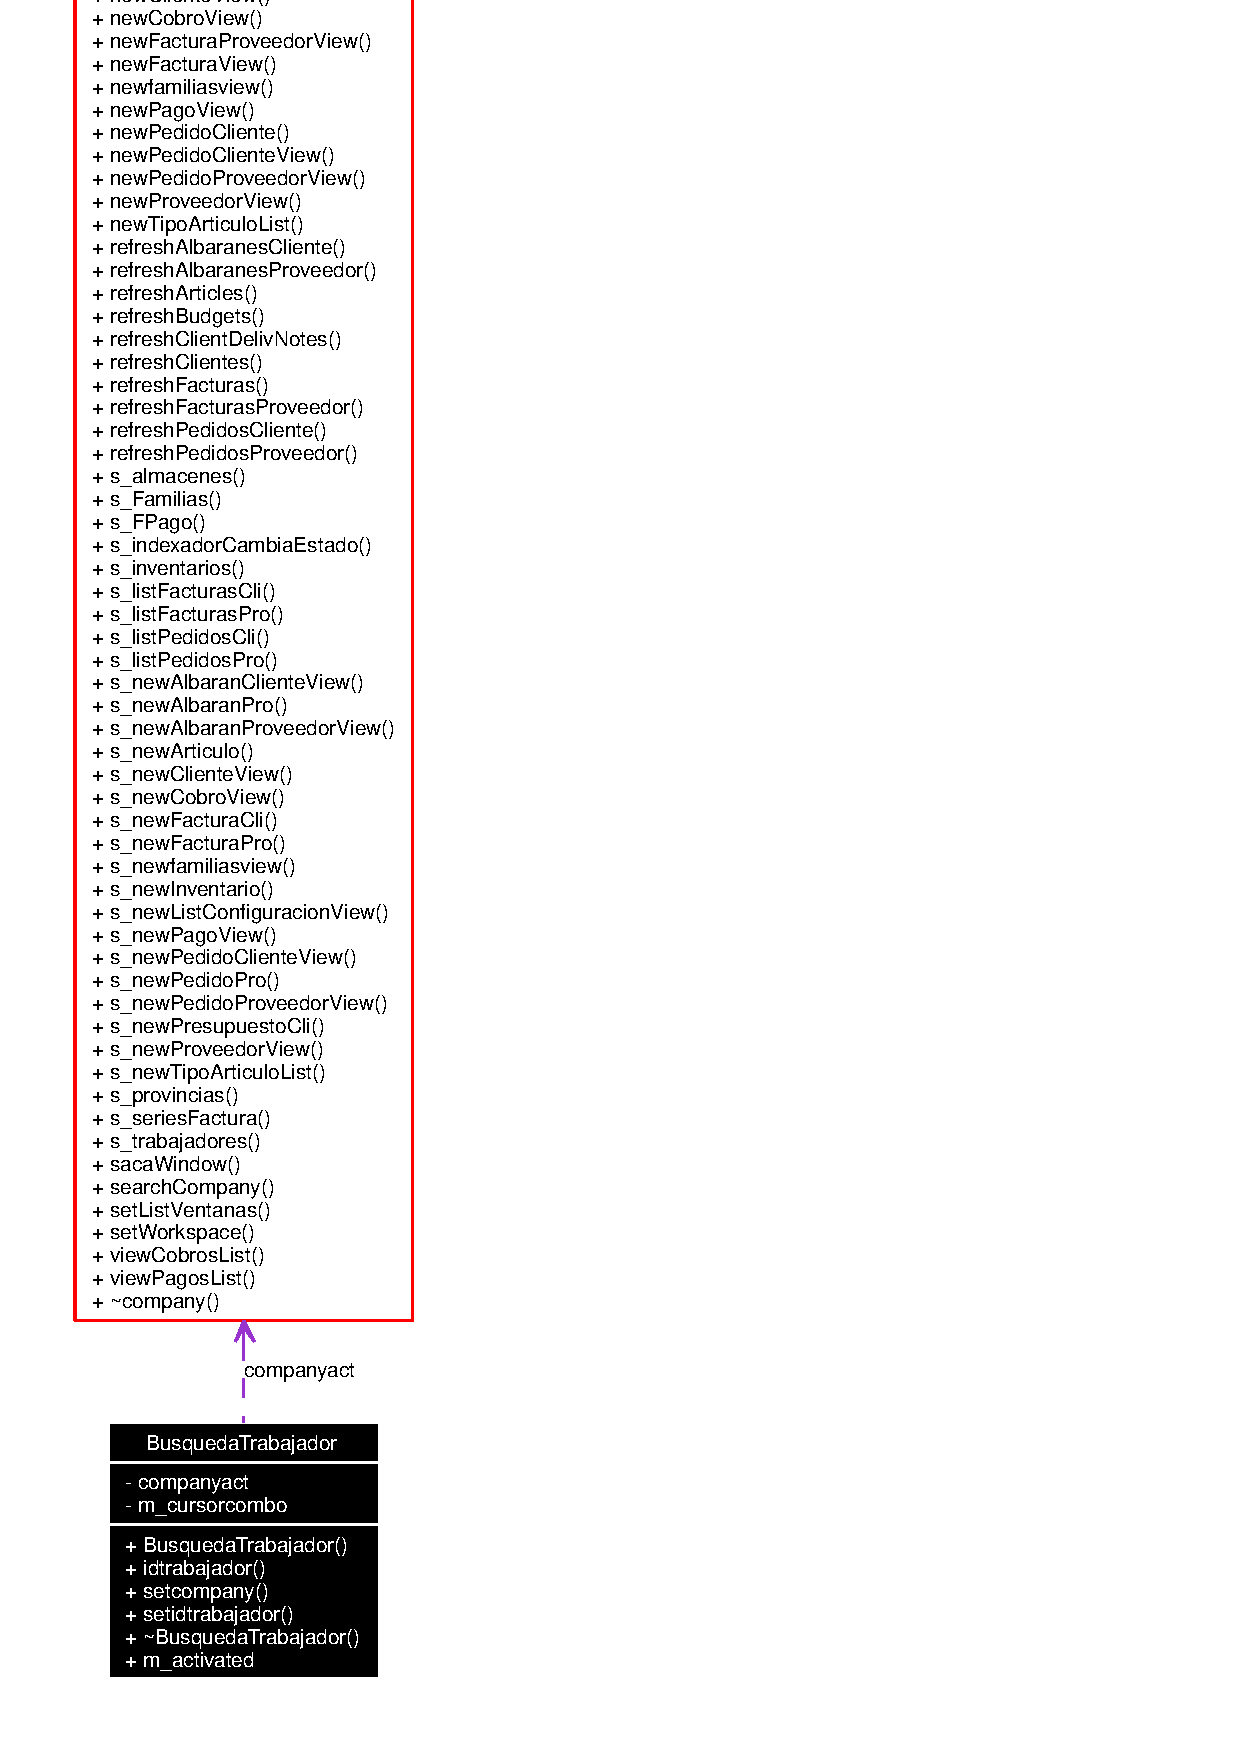
\includegraphics[width=99pt]{classBusquedaTrabajador__coll__graph}
\end{center}
\end{figure}
\subsection*{Slots p\'{u}blicos}
\begin{CompactItemize}
\item 
void {\bf m\_\-activated} (int index)\label{classBusquedaTrabajador_i0}

\end{CompactItemize}
\subsection*{Se\~{n}ales}
\begin{CompactItemize}
\item 
void {\bf value\-Changed} (QString)\label{classBusquedaTrabajador_l0}

\end{CompactItemize}
\subsection*{M\'{e}todos p\'{u}blicos}
\begin{CompactItemize}
\item 
{\bf Busqueda\-Trabajador} (QWidget $\ast$parent=0)\label{classBusquedaTrabajador_a0}

\item 
QString {\bf idtrabajador} ()\label{classBusquedaTrabajador_a1}

\item 
void {\bf setcompany} ({\bf company} $\ast$comp)\label{classBusquedaTrabajador_a2}

\item 
virtual void {\bf setidtrabajador} (QString idtrabajador)\label{classBusquedaTrabajador_a3}

\end{CompactItemize}


\subsection{Descripci\'{o}n detallada}
Permite buscar y seleccionar un trabajador. 

Muestra la parte del formulario que permite buscar y seleccionar un trabajador. Aparece en forma de desplegable. 



La documentaci\'{o}n para esta clase fu\'{e} generada a partir de los siguientes archivos:\begin{CompactItemize}
\item 
busquedatrabajador.h\item 
busquedatrabajador.cpp\end{CompactItemize}
